In this Alloy analysis, we chose to focus on the BikePath lifecycle. Specifically, we want to describe the evolution of a bike path over time, from the initial recording to the final publication, ensuring that data validation steps (Goal G4) are respected. \\
We point out that the initial state represents the moment a bike path is created but has not yet evolved through the system steps.

\subsection{Objectives}
The objective of this analysis is to verify the consistency of the \textit{Best Bike Paths} dynamic model. In particular, this model ensures that a bike path follows the mandatory sequence of states (\textit{Recording} $\rightarrow$ \textit{Processing} $\rightarrow$ \textit{Validation}) before being published. It also verifies that the owner of a bike path cannot change over time, even if the bike path entity is mutable. Finally, it ensures that obstacles detected during path creation can be filtered by the user during the validation phase, but become immutable once the bike path is published.


\subsection{Model Description}

The model defines the static entities (\texttt{User}, \texttt{Obstacle}) and the dynamic entity \texttt{BikePath}, whose state and relations evolve over time steps.

\begin{lstlisting}[language=Alloy, caption={Signatures and Facts defined in the Alloy model}, label={lst:alloy-model}]
// Users are static entities
sig User {
    var bikePaths: set BikePath
}

// Obstacles are static entities detected during bike path creation
sig Obstacle {}

// Enum defining the lifecycle steps of a bike path
enum Step { Recording, Processing, Validation, Published }

// A BikePath is linked to a single User and evolves through steps
var sig BikePath {
    var owner: one User,
    var currentStep: one Step,
    var obstacles: set Obstacle
}

// FACTS

// F1: A bike path always belongs to its owner's set
fact BikePathOwnership {
    always (all bp: BikePath | bp in bp.owner.bikePaths)
}

// F2: System Initialization
// In the first state, all existing bike paths must be in Recording
fact NewBikePath {
    all bp: BikePath | bp.currentStep = Recording
}

// F2b: Creation Constraint
// Logic: If a bike path exists in the next state but not now,
// it is a NEW bike path and must start in Recording.
fact BikePathsStartInRecording {
    always (
        all bp: BikePath' | (bp not in BikePath) implies bp.currentStep' = Recording
    )
}

// F3: The owner of a bike path never changes
fact ImmutableOwner {
    always (all bp: BikePath | (bp in BikePath') implies bp.owner' = bp.owner)
}

// F4: Helper function for state transitions
fun nextState[s: Step]: one Step {
    s = Recording  => Processing else
    s = Processing => Validation else
    s = Validation => Published else
    Published  // Published stays Published
}

// F5: Describes the progression of bike paths
// Bike paths either move to the next step or stay at the current step
fact StateProgression {
    always (
        all bp: BikePath | bp in BikePath' implies (
            bp.currentStep' = bp.currentStep or
            bp.currentStep' = nextState[bp.currentStep]
        )
    )
}

// F5b: Sequential Integrity
// Explicitly forbids skipping steps to satisfy strict ordering requirements
fact NoSkippingSteps {
    always (all bp: BikePath | (bp in BikePath and bp in BikePath') implies (
        (bp.currentStep = Recording) implies 
            (bp.currentStep' = Recording or bp.currentStep' = Processing)
        and
        (bp.currentStep = Processing) implies 
            (bp.currentStep' = Processing or bp.currentStep' = Validation)
        and
        (bp.currentStep = Validation) implies 
            (bp.currentStep' = Validation or bp.currentStep' = Published)
        and
        (bp.currentStep = Published) implies bp.currentStep' = Published
    ))
}

// F6: Obstacle Consistency
fact ObstacleConstraint {
    always (all bp: BikePath | bp in BikePath' implies (
        // Once published, obstacles are immutable
        (bp.currentStep = Published implies bp.obstacles' = bp.obstacles)
        and
        // Obstacles cannot be added during Processing or Validation, only removed
        (bp.currentStep in Processing + Validation implies 
            bp.obstacles' in bp.obstacles)
    ))
}

// F7: Liveness
fact EndBikePath {
    all bp: BikePath | eventually (bp not in BikePath or bp.currentStep = Published)
}
\end{lstlisting}

\subsection{Analysis and Validation}

To validate the model, we use \textbf{Predicates} to generate valid scenarios and \textbf{Assertions} to verify that no invalid states are reachable.

\subsubsection{Predicates}

\textbf{Example 1: Correct Path Scenario}

In this example, we verify a typical lifecycle: a bike path is created, goes through \texttt{Recording}, \texttt{Processing}, waits for \texttt{Validation}, and finally reaches the \texttt{Published} state.

\begin{lstlisting}[language=Alloy, caption={Predicate: Complete BikePath Lifecycle}]
pred show[] {
    #BikePath = 0
    // Eventually a bike path is created
    eventually (#BikePath = 1)
    // Eventually the bike path reaches the Published state
    eventually (some bp: BikePath | bp.currentStep = Published)
}
run show for 6
\end{lstlisting}

\begin{figure}[H]
    \centering
    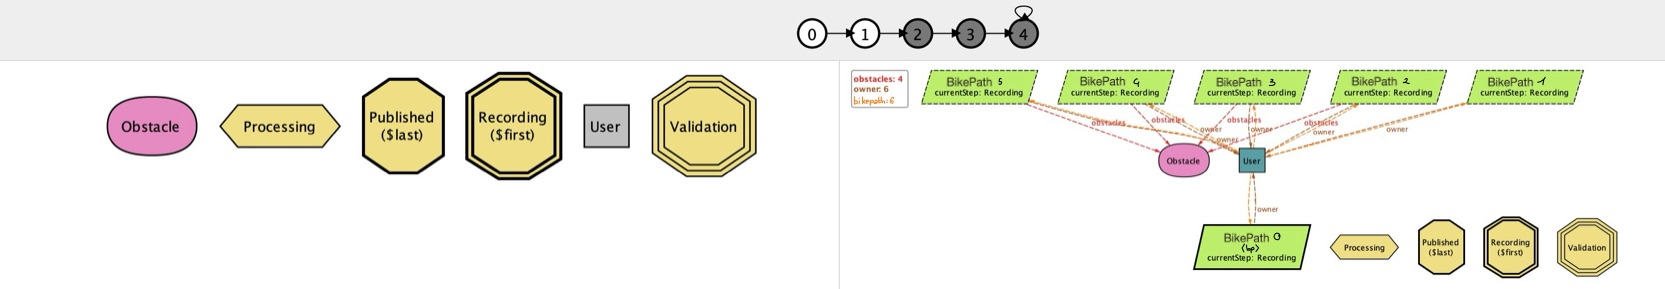
\includegraphics[width=0.9\textwidth]{RASD/images/alloy101.png}
    \caption{Time 0-1.}
    \label{fig:alloy-ex1-01}
\end{figure}
\noindent
At \textbf{Time 0}, the system is in a quiescent state with the User present but no active paths. Transitioning to \textbf{Time 1}, the User initiates bike path creation. The model generates a new \texttt{BikePath} instance and links it to the User (\texttt{owner}). As constrained by the \texttt{NewBikePath} fact, the system strictly initializes the bike path's state to \texttt{Recording}, representing the start of GPS and sensor data acquisition.

\begin{figure}[H]
    \centering
    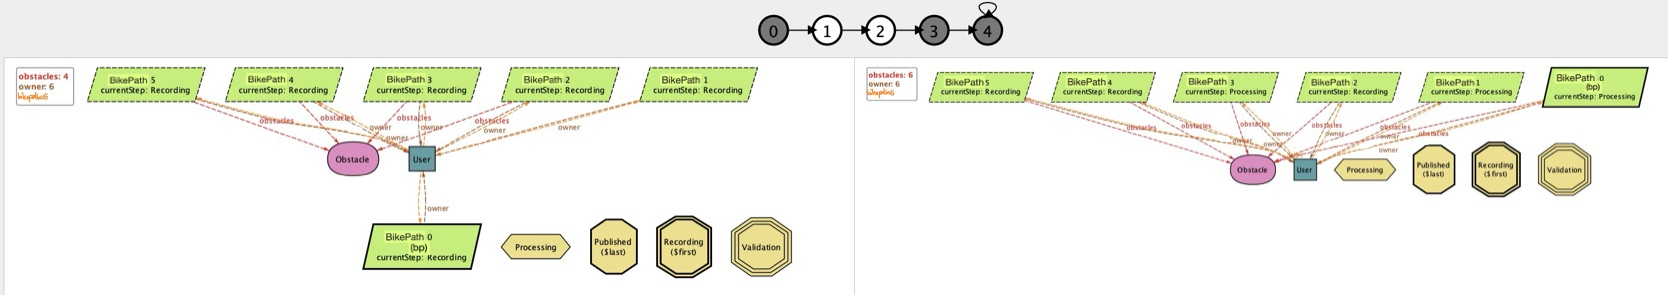
\includegraphics[width=0.9\textwidth]{RASD/images/alloy112.png}
    \caption{Time 1-2.}
    \label{fig:alloy-ex1-12}
\end{figure}
\noindent
The model illustrates the evolution of concurrent bike path creation sessions. While \texttt{BikePath2} through \texttt{BikePath5} persist in the \texttt{Recording} phase, \texttt{BikePath0} and \texttt{BikePath1} advance to the \texttt{Processing} state. This transition validates the \texttt{StateProgression} fact, ensuring that the lifecycle proceeds sequentially from raw data collection to the analysis phase without skipping mandatory steps.

\begin{figure}[H]
    \centering
        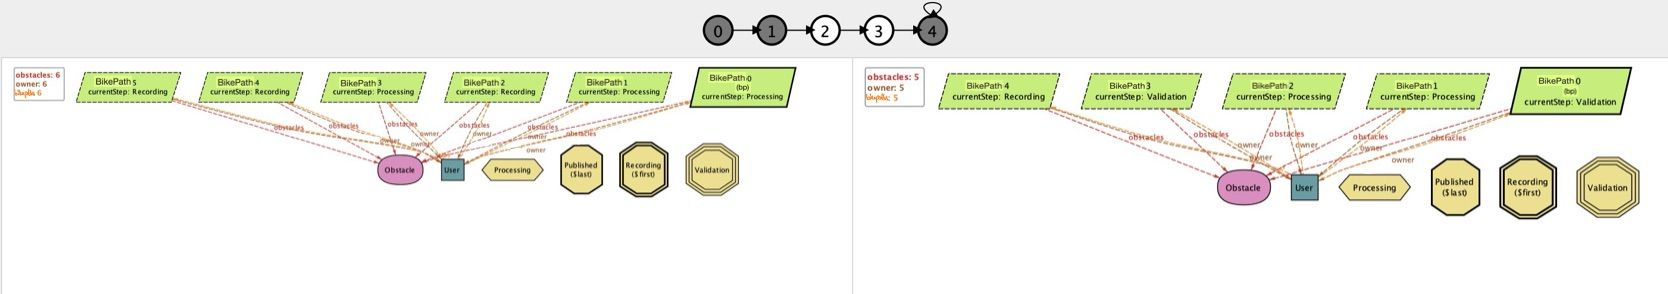
\includegraphics[width=0.9\textwidth]{RASD/images/alloy123.png}
    \caption{Time 2-3.}
    \label{fig:alloy-ex1-23}
\end{figure}
\noindent
In the transition to the third state, the model exhibits further lifecycle advancements alongside entity dynamics. \texttt{BikePath0} and \texttt{BikePath3} progress to the \texttt{Validation} phase, while \texttt{BikePath2} moves to \texttt{Processing}. Notably, \texttt{BikePath5} is removed from the system, decreasing the total bike path count.

\begin{figure}[H]
    \centering
    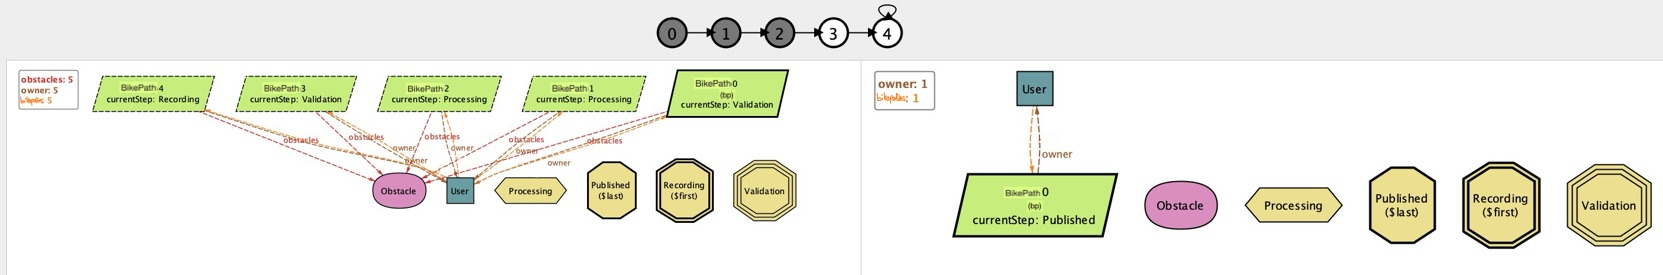
\includegraphics[width=0.9\textwidth]{RASD//images/alloy134.png}
    \caption{Time 3-4.}
    \label{fig:alloy-ex1-34}
\end{figure}
\noindent
In the final stage, the system reaches the target state. \texttt{BikePath0} successfully transitions from \texttt{Validation} to \texttt{Published}, marking the completion of the bike path creation process and making it available to the community.

\clearpage
\textbf{Example 2: BikePath Discarded}

This example illustrates a scenario where the user is not satisfied with the collected data. The bike path progresses correctly to the \texttt{Validation} phase, but then it is removed from the system instead of moving to \texttt{Published}.

\begin{lstlisting}[language=Alloy, caption={Predicate: Discarding a BikePath}]
pred discardedAfterRecording[] {
    eventually (some bp: BikePath | 
        bp.currentStep = Validation and 
        // The bike path disappears in the next state
        (bp not in BikePath') 
    )
}
run discardedAfterRecording for 6
\end{lstlisting}

\begin{figure}[H]
    \centering
    
\includegraphics[width=0.9\textwidth]{RASD//images/alloy201.png}
    \caption{Time 0-1.}
    \label{fig:alloy-ex2-01}
\end{figure}
\noindent
In the initial phase of the discard scenario, all bike paths start in the \texttt{Recording} state. Moving to the next step, the instance marked for future removal (\texttt{BikePath2}), along with others, correctly transitions to \texttt{Processing}.

\begin{figure}[H]
    \centering
    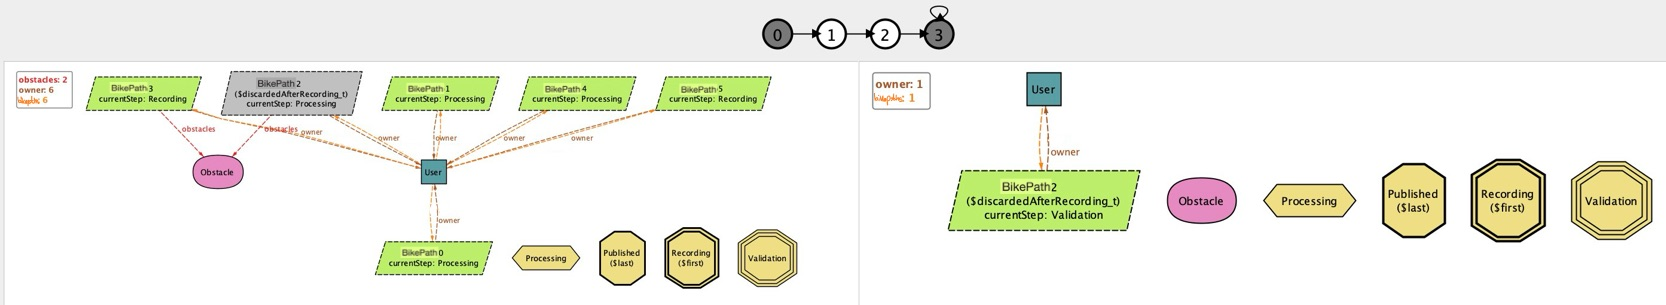
\includegraphics[width=0.9\textwidth]{RASD//images/alloy212.png}
    \caption{Time 1-2.}
    \label{fig:alloy-ex2-12}
\end{figure}
\noindent
In this phase, the targeted instance (\texttt{BikePath2}) progresses from \texttt{Processing} to the \texttt{Validation} state.
\clearpage

\textbf{Example 3: Removing False Positives}

As shown in the model, during the validation step, the user can filter the data. This example represents the removal of "false positives" detected by sensors: the set of obstacles shrinks before the bike path becomes public.

\begin{lstlisting}[language=Alloy, caption={Predicate: Obstacle Refinement}]
pred falsePositiveRemoval[] {
    some bp: BikePath | eventually (
        bp.currentStep = Validation and
        // The number of obstacles decreases in the next step
        #bp.obstacles' < #bp.obstacles and
        bp.currentStep' = Published
    )
}
run falsePositiveRemoval for 6
\end{lstlisting}
\begin{figure}[H]
    \centering
    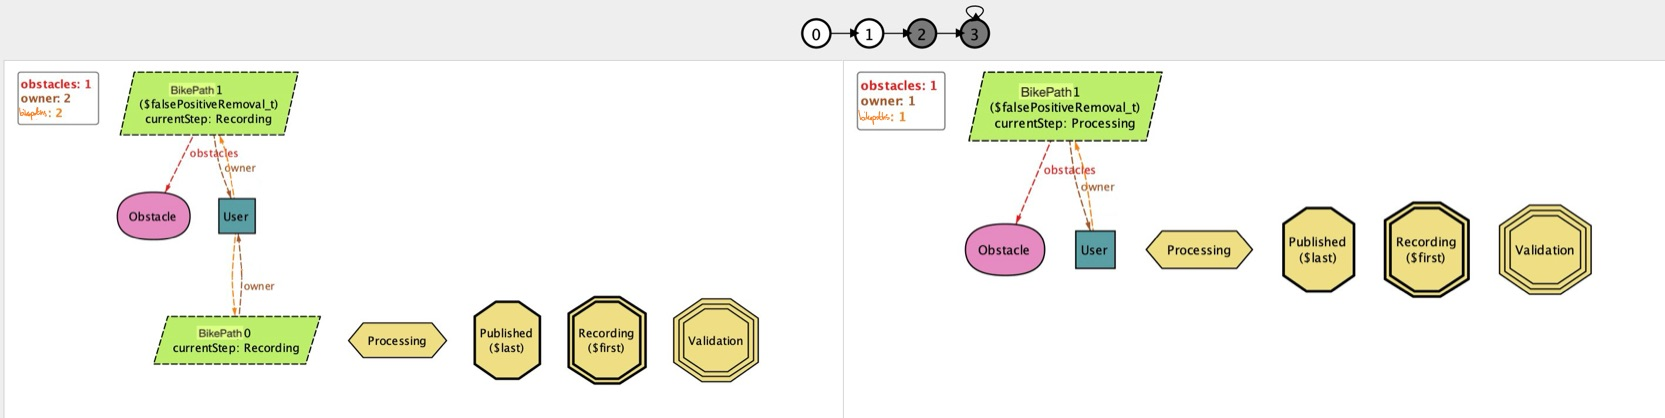
\includegraphics[width=0.9\textwidth]{RASD//images/alloy301.png}
    \caption{Time 0-1.}
    \label{fig:alloy-ex3-01}
\end{figure}
\noindent
In the setup for the obstacle refinement scenario, the target instance \texttt{BikePath1} begins in the \texttt{Recording} state with associated obstacles. Transitioning to the next step, the bike path advances to \texttt{Processing}.

\begin{figure}[H]
    \centering
    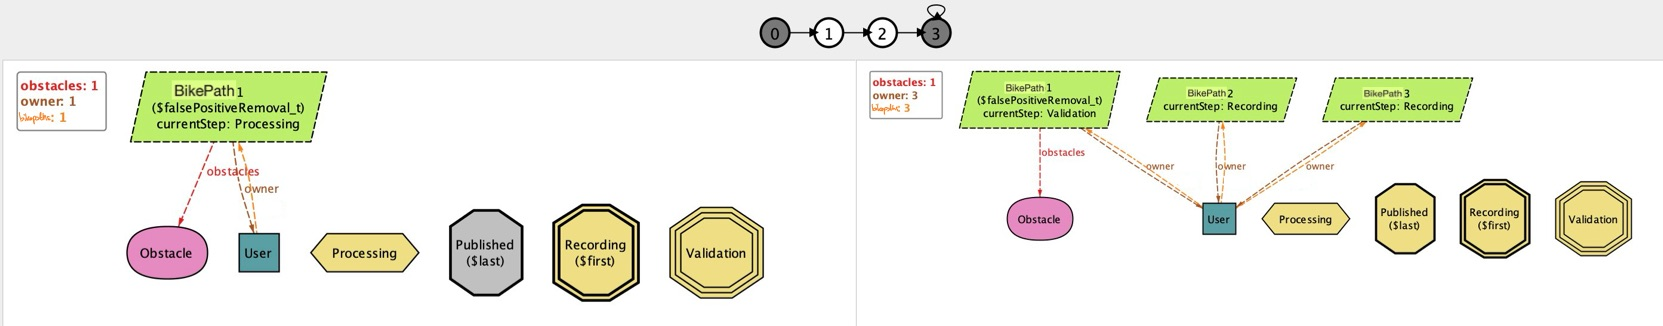
\includegraphics[width=0.9\textwidth]{RASD//images/alloy312.png}
    \caption{Time 1-2.}
    \label{fig:alloy-ex3-12}
\end{figure}
\noindent
In this transition, \texttt{BikePath1} advances to the \texttt{Validation} phase, establishing the necessary context for the user to review and filter detected anomalies. Concurrently, the system demonstrates its dynamic capacity by initializing new path creation sessions (\texttt{BikePath2} and \texttt{BikePath3}) in the \texttt{Recording} state.

\begin{figure}[H]
    \centering
    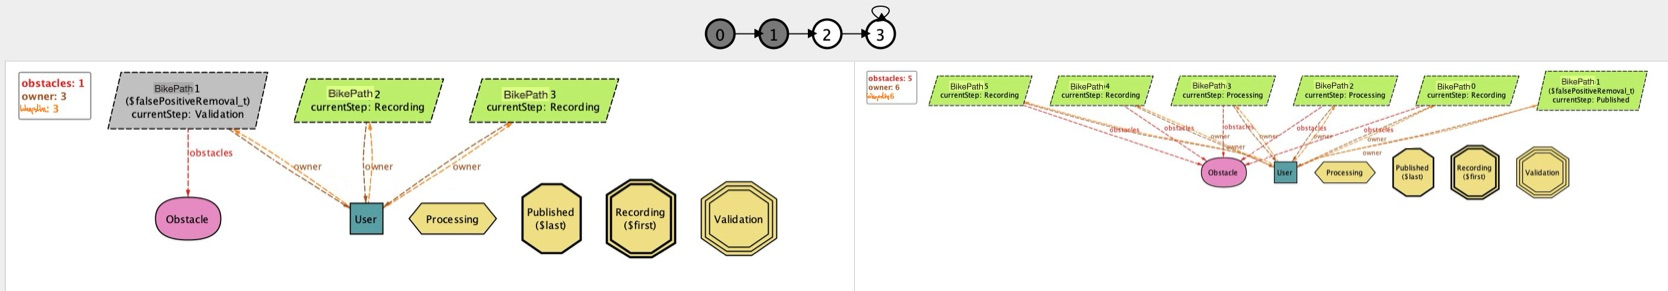
\includegraphics[width=0.9\textwidth]{RASD//images/alloy323.png}
    \caption{Time 2-3.}
    \label{fig:alloy-ex3-23}
\end{figure}
\noindent
\texttt{BikePath1} transitions from \texttt{Validation} to \texttt{Published}. The association with the detected \texttt{Obstacle} is severed. This reduction in the set of linked obstacles satisfies the \texttt{falsePositiveRemoval} predicate.
\clearpage

\subsubsection{Assertions}

Finally, through assertions, we verify critical safety properties. The checks confirm that strictly invalid behaviors are impossible in our model.

\textbf{Assertion 1: No Skipped Steps}

We ensure that every published bike path has strictly followed the mandatory lifecycle (Recording $\rightarrow$ Processing $\rightarrow$ Validation $\rightarrow$ Published).

\begin{lstlisting}[language=Alloy, caption={Assertion: Safety Check for Steps}]
assert noSkippedSteps {
    always (all bp: BikePath |
        bp.currentStep = Published implies
        (once bp.currentStep = Validation) and
        (once bp.currentStep = Recording)
        )
}
check noSkippedSteps for 8
\end{lstlisting}

\begin{figure}[H]
    \centering
    
\includegraphics[width=0.9\textwidth]{RASD//images/alloy4.png}
    \caption{}
    \label{fig:alloy-ex4}
\end{figure}

\clearpage
\textbf{Assertion 2: Immutable Published State}

We verify that once a bike path reaches the \texttt{Published} state, it cannot revert to a previous state or change its status.

\begin{lstlisting}[language=Alloy, caption={Assertion: Published Persistence}]
assert publishedStaysPublished {
    always (all bp: BikePath |
        (bp.currentStep = Published and bp in BikePath') implies
            bp.currentStep' = Published
    )
}
check publishedStaysPublished for 8
\end{lstlisting}

\begin{figure}[H]
    \centering
    
\includegraphics[width=0.9\textwidth]{RASD//images/alloy5.png}
    \caption{}
    \label{fig:alloy-ex5}
\end{figure}

\clearpage
\textbf{Assertion 3: Immutable Owner}

We verify that the owner of a bike path cannot change over time, ensuring data integrity and preventing unauthorized transfers of ownership.

\begin{lstlisting}[language=Alloy, caption={Assertion: Owner persistence}]
assert ownerImmutable {
    always (all bp: BikePath |
        bp in BikePath' implies bp.owner' = bp.owner
    )
}
check ownerImmutable for 8
\end{lstlisting}

\begin{figure}[H]
    \centering
    
\includegraphics[width=0.9\textwidth]{RASD//images/alloy6.png}
    \caption{}
    \label{fig:alloy-ex6}
\end{figure}